\chapter{Experimentos}\label{cap:experimentos}

\section{Base de dados}

A base de dados (imagens) utilizada advém do projeto GEOMA \cite{geoma}, financiado pelo Instituto de Pesquisas Espaciais (INPE). Trata-se de imagens coloridas, codificadas em JPEG e com 640 pixels de largura por 480 pixels de altura. A base é composta por fotografias ortogonais ao relevo (como pode ser visto na figura \ref{fig:amostra}), de altitudes variadas e tiradas a partir de aeronaves tripuladas, durante o trajeto entre diversas cidades da região amazônica.

No momento do início dos experimentos deste trabalho, estas imagens tiradas de aviões tripulados eram as únicas disponíveis publicamente. Podemos considerá-las válidas por terem sido tiradas em altitude de voo compatível com as missões de VANTs de vigilância, entre 900 e 1.100 metros do solo. Como este trabalho tem como objetivo utilizar apenas câmeras de espectro visível, são dispensáveis comparações de sensores com VANTs que eventualmente possuam sonar, câmeras infravermelho ou outros tipos de sensores.

\begin{figure}[h]
  \centering
  \begin{subfigure}[b]{0.3\textwidth}
    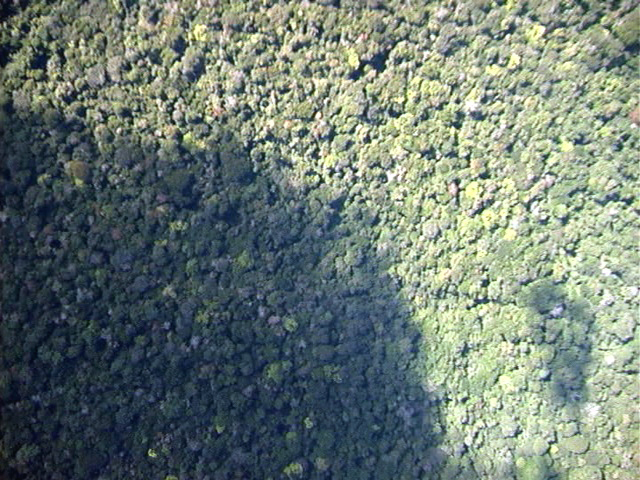
\includegraphics[width=\textwidth]{imgs/amostra1}
  \end{subfigure}%
  ~
  \begin{subfigure}[b]{0.3\textwidth}
    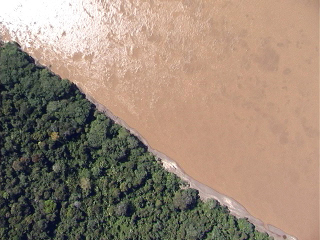
\includegraphics[width=\textwidth]{imgs/amostra2}
  \end{subfigure}%
  ~
  \begin{subfigure}[b]{0.3\textwidth}
    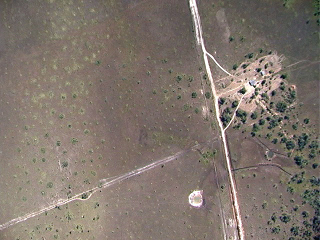
\includegraphics[width=\textwidth]{imgs/amostra3}
  \end{subfigure}%
  \caption{Amostras da base de dados}
  \label{fig:amostra}
\end{figure}

A base possui um total de 3.044 imagens, com dimensão total de 1,02 Gigabytes de dados. Cerca de 150 imagens foram utilizadas nos experimentos até o momento, visto que um grande esforço precisa ser despendido na classificação manual das imagens em todas as etapas do experimento, consumindo um tempo considerável.

Para criar uma referência (\textit{ground-truth}) para a segmentação das imagens da base de dados, uma ferramenta computacional executável em navegadores web foi construída (figura \ref{fig:manualseg}). A saída deste aplicativo é uma coleção, para cada imagem, de informações sobre bordas das regiões da imagem. Estas informações servirão de referência para avaliar o desempenho dos algoritmos de segmentação testados neste trabalho.

\begin{figure}[h]
  \centering
  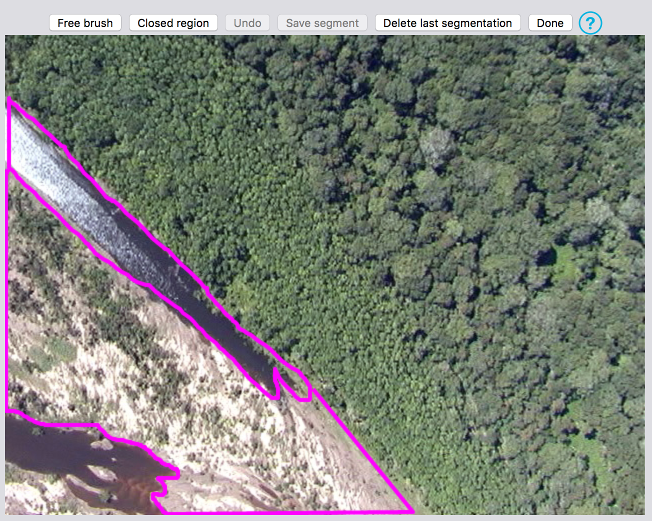
\includegraphics[width=0.7\textwidth]{imgs/manualseg}
  \caption{Ferramenta para segmentação manual das imagens}
  \label{fig:manualseg}
\end{figure}

\section{Segmentação}

Um experimento de comparação entre diversos algoritmos de segmentação de imagens foi planejado. Cada imagem da base de dados foi segmentada por seres humanos, segmentações estas que constituíram a base de referência para o experimento. Cada imagem tem sua segmentação de referência consolidada a partir da segmentação manual de pelo menos 5 seres humanos.

\subsection{Protocolo experimental}

Para criação da segmentação manual de referência (\textit{ground-truth}), 31 voluntários, todos alunos de pós-graduação em informática ou áreas relacionadas, foram convidados a realizar a segmentação manual das imagens da base de dados, através de uma ferramenta\footnote{http://amazonsegmentation.ddns.net/} criada com esta finalidade. A ferramenta de software web criada consiste de uma interface gráfica onde o usuário pode desenhar sobre uma imagem a ser segmentada. A ideia é que nesta imagem sejam circunscritas as bordas das regiões definidas pelo usuário, de acordo com instruções fornecidas pela ferramenta e que foram lidas obrigatoriamente por cada voluntário antes do início do experimento.

Em linhas gerais, as instruções orientam os participantes no experimento a segmentar as imagens de acordo com a cobertura ou tipo de terreno, formação geológica ou vegetação, utilizando os critérios e granularidade que lhes pareçam mais adequados:

\begin{citacao}[english]
Your mission is to manually segment the given images as accurately as possible, according to your own judgment. The criteria here is terrain coverage. So, we would like to separate different vegetations, geological formations and human-made objects \cite{amazonsegmentation}
\end{citacao}

O conteúdo integral das instruções pode ser encontrado no apêndice \ref{apendice:instrucoesManualSeg}.

%TODO O que se faz para unir e consolidar as segmentações?
%TODO Este método foi proposto por quem?
%TODO Qual a base estatística?

\subsection{Métricas}

%TODO Lugar certo? Talvez deva estar junto às métricas de avaliação de machine learning, na seção de fundamentação teórica, subseção de avaliação

Em primeiro lugar, é preciso aferir a validade da base de dados de segmentações manuais (\textit{ground-truth}), demonstrando que segmentações de uma mesma imagem feitas por diferentes indivíduos são consistentes. Em um segundo momento, é preciso avaliar os algoritmos de segmentação de forma objetiva.

O problema em mensurar a consistência entre duas segmentações é que não há uma única segmentação possível para uma imagem. Duas pessoas podem segmentar uma imagem de forma significativamente diferente por terem uma percepção diferente da cena, ou ainda, por usar diferentes granularidades na segmentação.

Quando a diferença entre duas segmentações advém de uma diferença de percepção da cena, é esperado que o erro seja grande e que as segmentações sejam consideradas inconsistentes. Quando a diferença é de granularidade, uma segmentação pode ser considerada apenas um refinamento da outra, portanto, o erro deve ser baixo ou até zero \cite{martin:2001}.

%TODO Adicionar uma imagem para demonstrar diferenças de granularidade?

Segmentação de imagens é simplesmente a divisão de pixels de uma imagem em conjuntos (segmentos). Uma possível medida de erro tem como entrada duas segmentações, $S_1$ e $S_2$, e tem como saída um valor real no intervalo $[0...1]$, onde $0$ significa ausência de erros de segmentação.

Ainda de acordo com o trabalho de \citeonline{martin:2001}, é necessário utilizar medidas que sejam lenientes com o refinamento de granularidade entre duas segmentações de uma mesma imagem. Entende-se que se os pixels de um segmento podem ser considerados um subconjunto adequado de um outro segmento, trata-se de um refinamento e o erro deve ser zero. Se não existe relação de subconjunto entre os segmentos, as regiões devem ser consideradas inconsistentes e o erro deve ser significativo.

Se $R(S,p_i)$ é o conjunto de pixels correspondentes a uma região na segmentação $S$ que contém o pixel $p_i$, onde $\setminus$ denota o conjunto complementar, o erro de refinamento local é definido por:

\begin{equation}
	E(S_1,S_2,p_i) = \frac{|R(S_1,p_i) \setminus R(S_2,p_i)|}{|R(S_1,p_i)|}
\end{equation}


A partir desta relação, \citeonline{martin:2001} define duas métricas de erro de segmentação: Erro de Consistência Global (Global Consistency Error, ou GCE) e Erro de Consistência Local (Local Consistency Error, ou LCE):

\begin{equation}
	GCE(S_1,S_2) = \frac{1}{n} min \biggl\{ \sum_{i} E(S_1,S_2,p_i), \sum_{i} E(S_2,S_1,p_i) \biggr\}
\end{equation}

\begin{equation}
	LCE(S_1,S_2) = \frac{1}{n} \sum_{i} min \biggl\{ E(S_1,S_2,p_i), E(S_2,S_1,p_i) \biggr\}
\end{equation}

Uma vez que $LCE \geq GCE$ entre segmentações de uma mesma imagem, é correto afirmar que $GCE$ é uma medida mais rígida que $LCE$. Além dos casos em que uma segmentação é um refinamento de outra, há ainda dois casos em que o erro de segmentação pode ser zero: quando os segmentos são compostos por apenas um pixel cada ou quando toda a imagem é composta de apenas um segmento.

\subsection{Resultados}

Antes de analisar o desempenho de cada algoritmo de segmentação presente neste trabalho em relação à segmentação manual, é preciso aferir a validade da própria segmentação manual, visto que ela foi realizada por diferentes participantes. Segundo \citeonline{martin:2001}, uma forma de validar a consistência das segmentações manuais é medir o erro entre segmentações de uma mesma imagem feita por diferentes pessoas.

Utilizando as métricas de erro de consistência local (LCE) e global (GCE) para medir a similaridade das segmentações manuais, os resultados confirmam a consisência da segmentação manual feira pelos participantes do experimento. Conforme pode ser visto nas figuras \ref{fig:manual_gce} e \ref{fig:manual_lce}, os coeficientes de erro global e local, respectivamente, ficam abaixo dos 20\% e 10\% para todos os casos.

\begin{figure}[h]
  \centering
  \begin{subfigure}[b]{0.5\textwidth}
    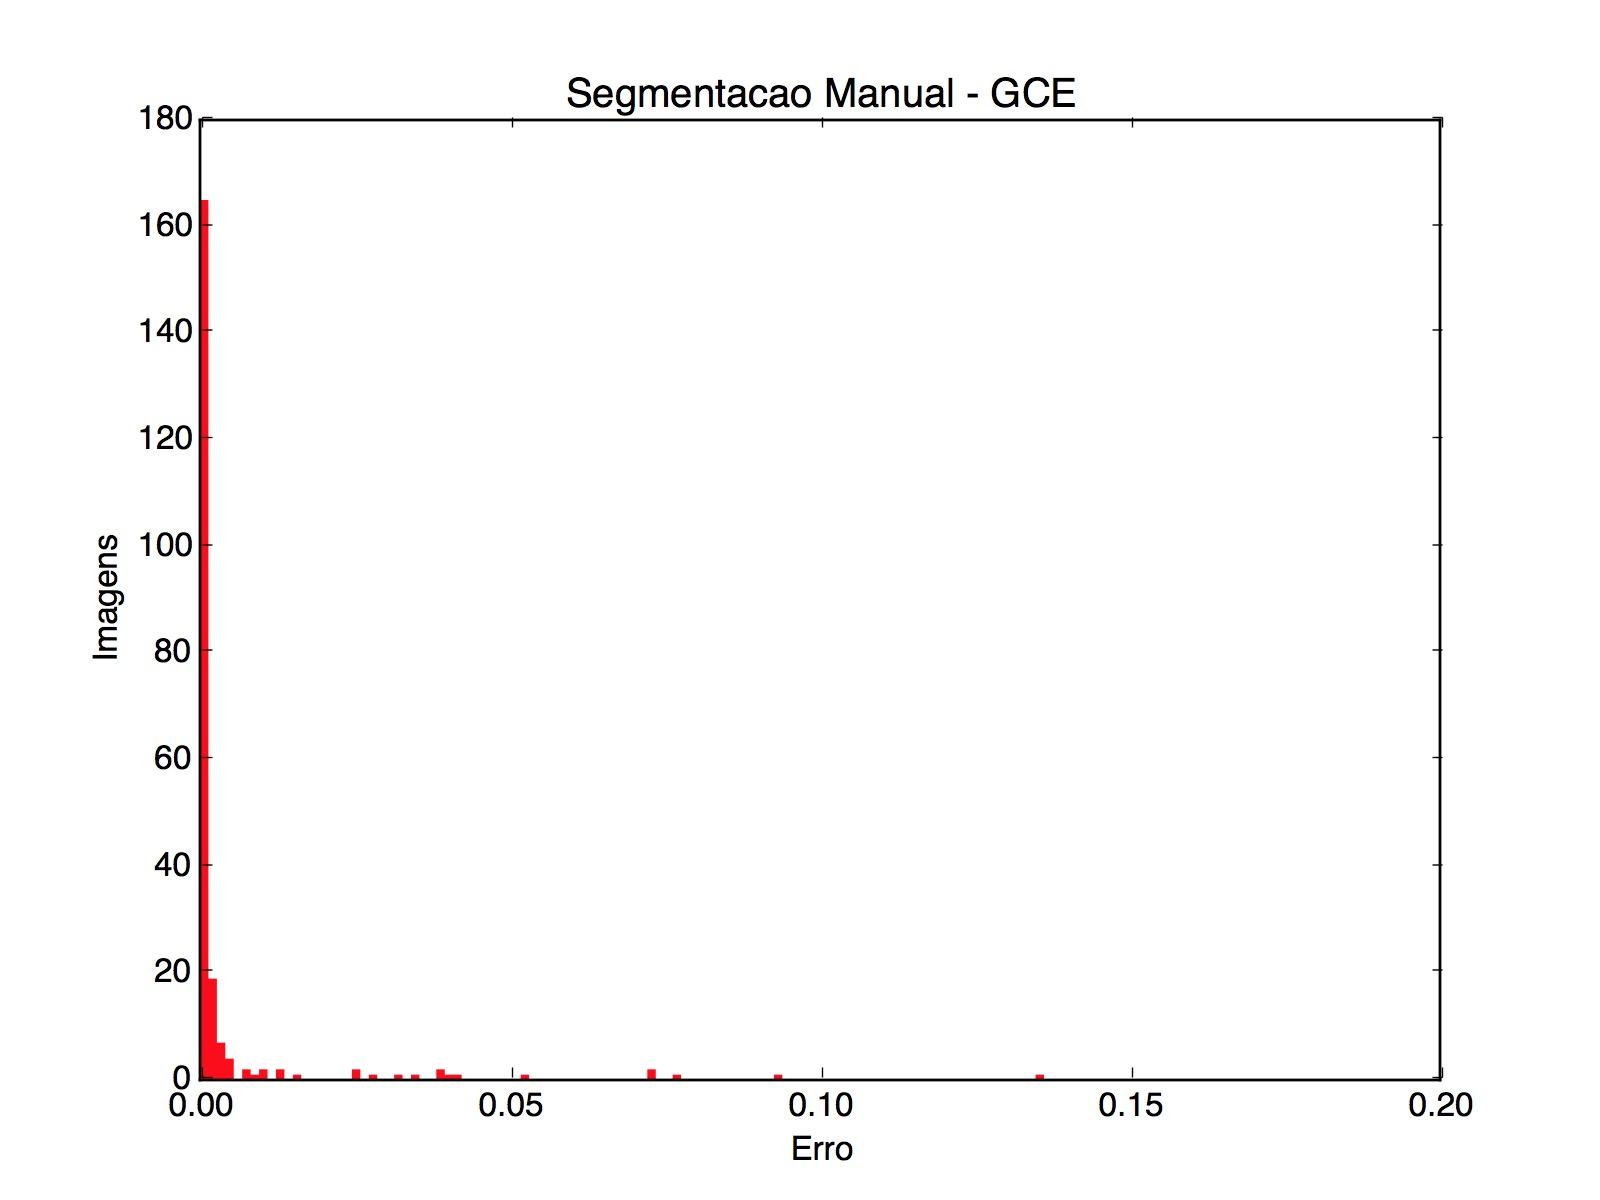
\includegraphics[width=\textwidth]{imgs/manual_gce}
  \end{subfigure}%
  ~
  \begin{subfigure}[b]{0.5\textwidth}
    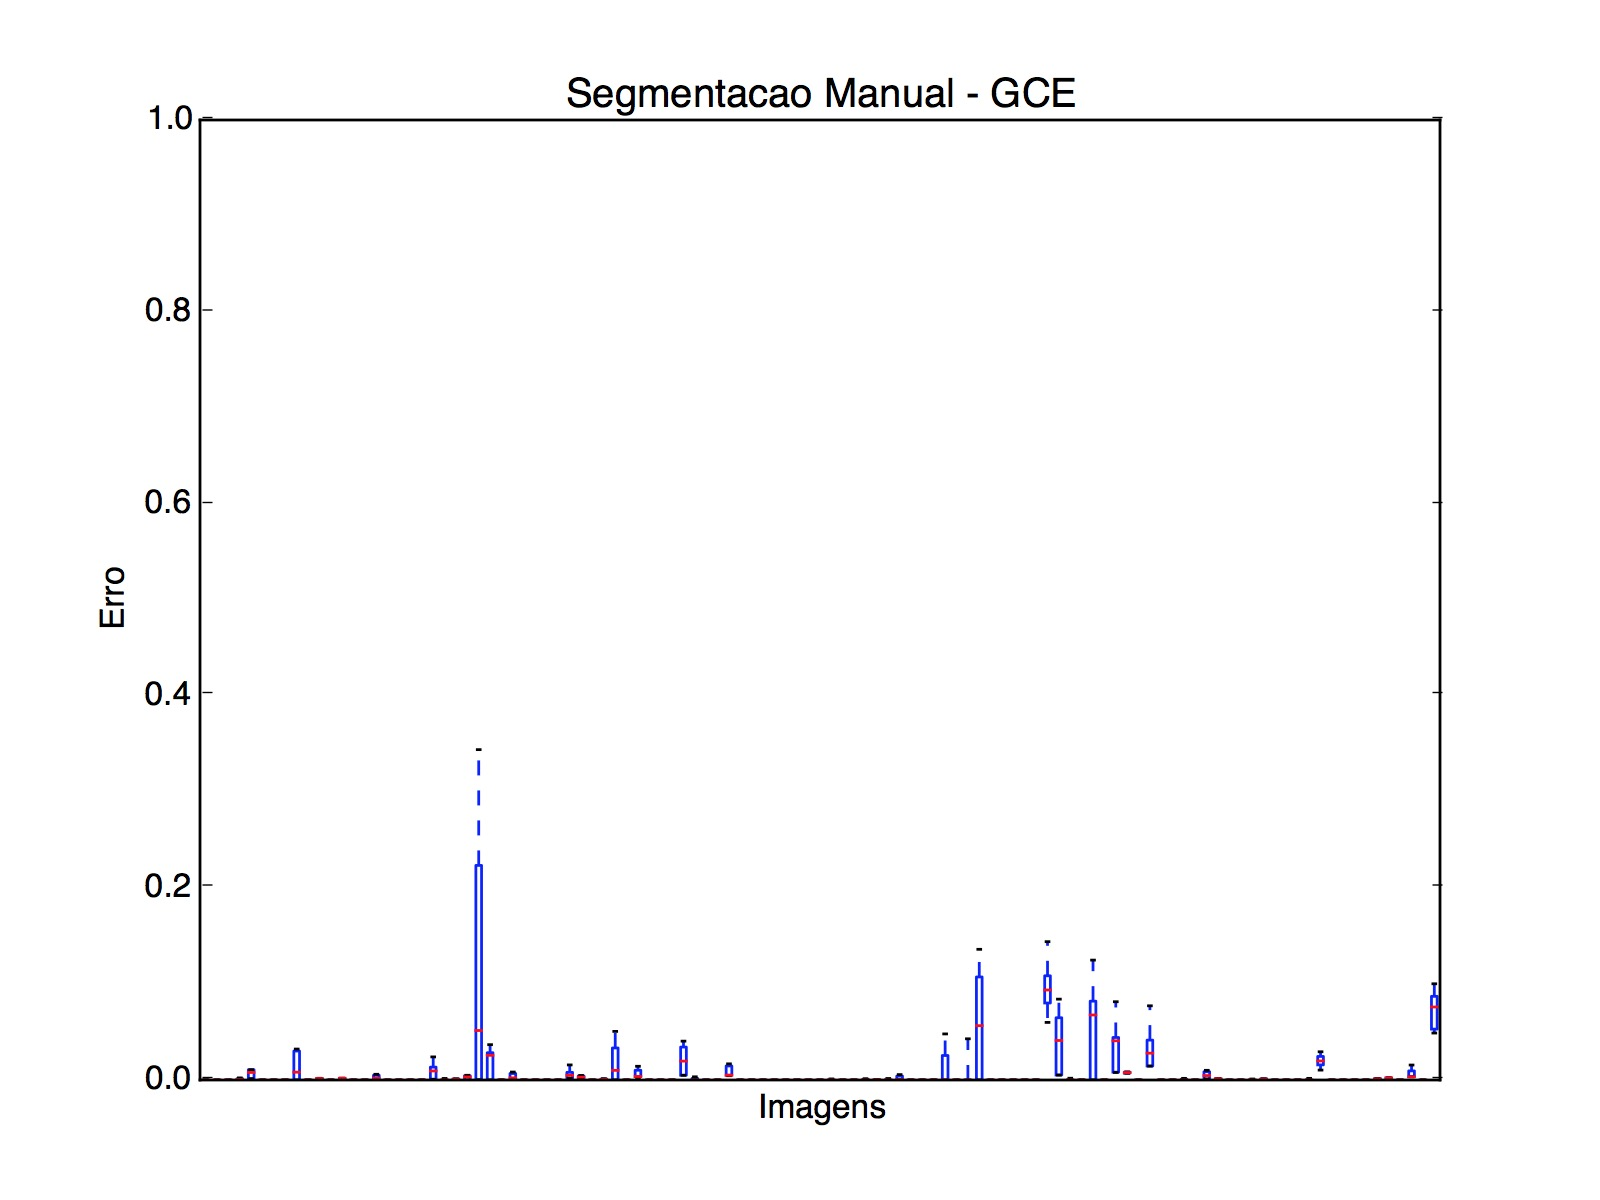
\includegraphics[width=\textwidth]{imgs/manual_dist_gce}
  \end{subfigure}%
  \caption{Coeficiente de erro global das diferentes segmentações de mesma imagem}
  \label{fig:manual_gce}
\end{figure}

\begin{figure}[h]
  \centering
  \begin{subfigure}[b]{0.5\textwidth}
    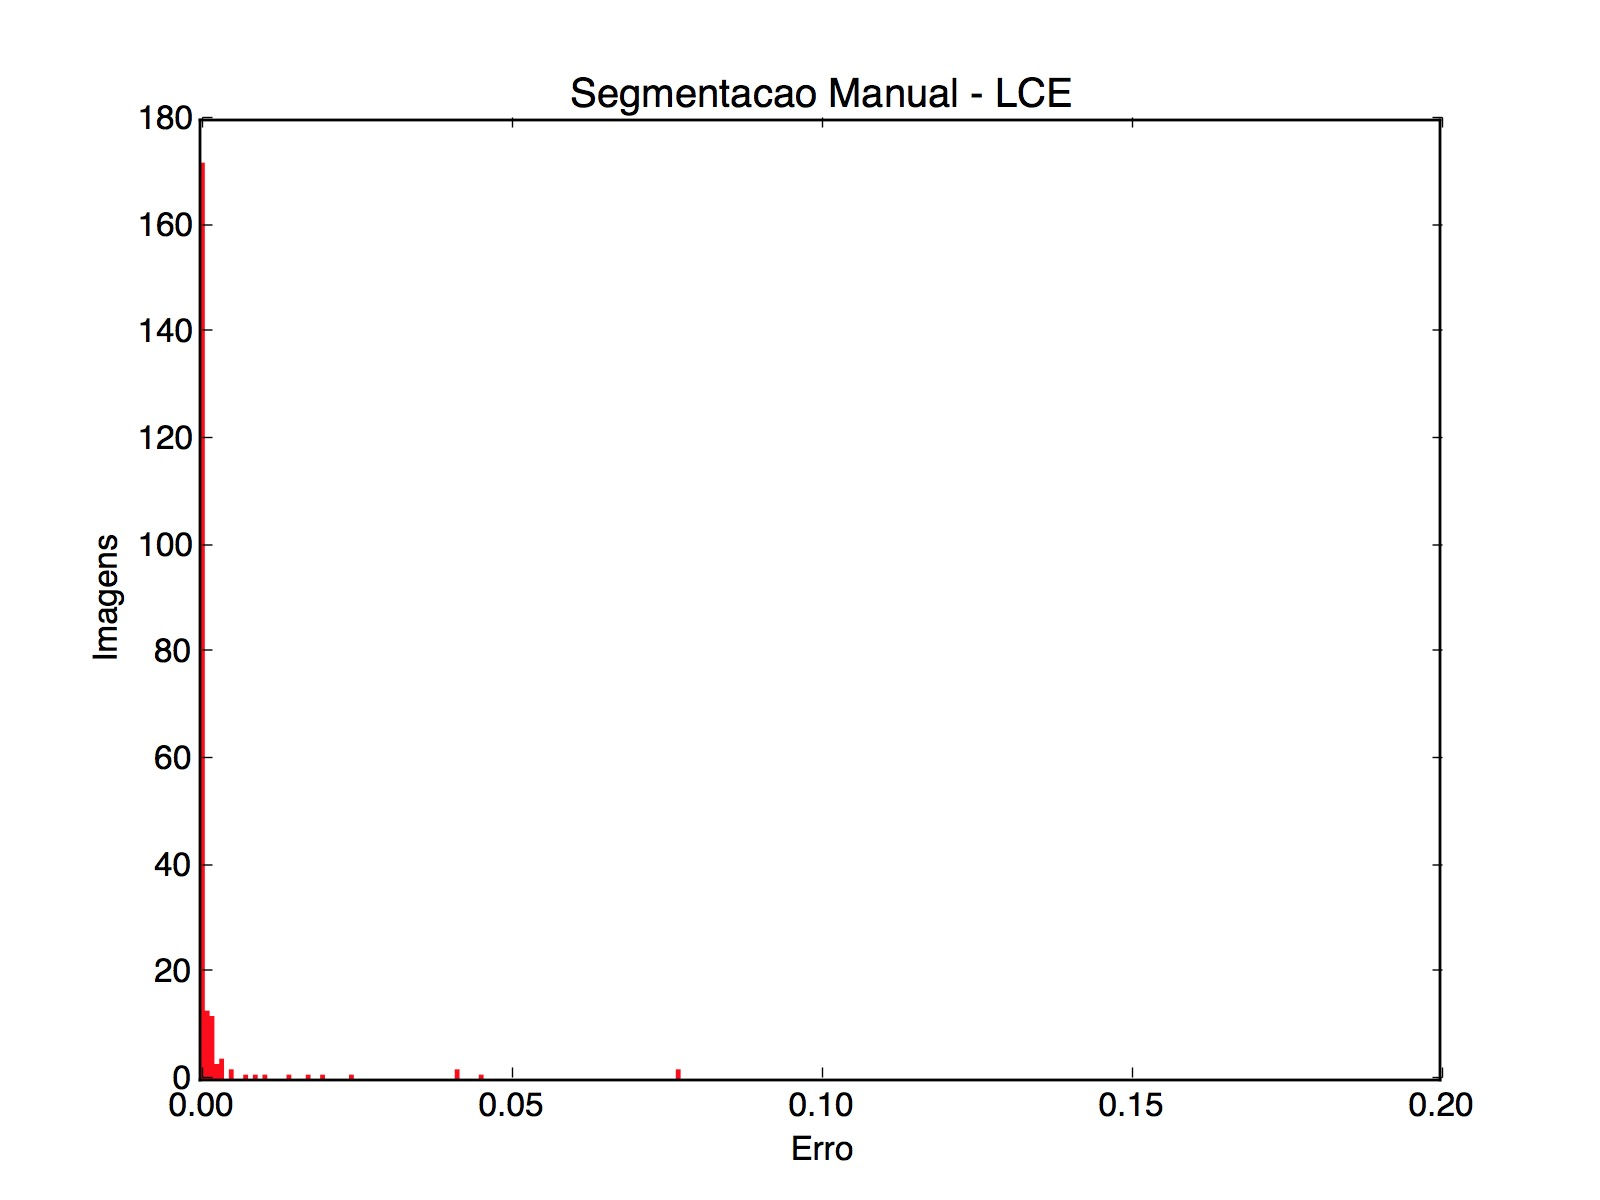
\includegraphics[width=\textwidth]{imgs/manual_lce}
  \end{subfigure}%
  ~
  \begin{subfigure}[b]{0.5\textwidth}
    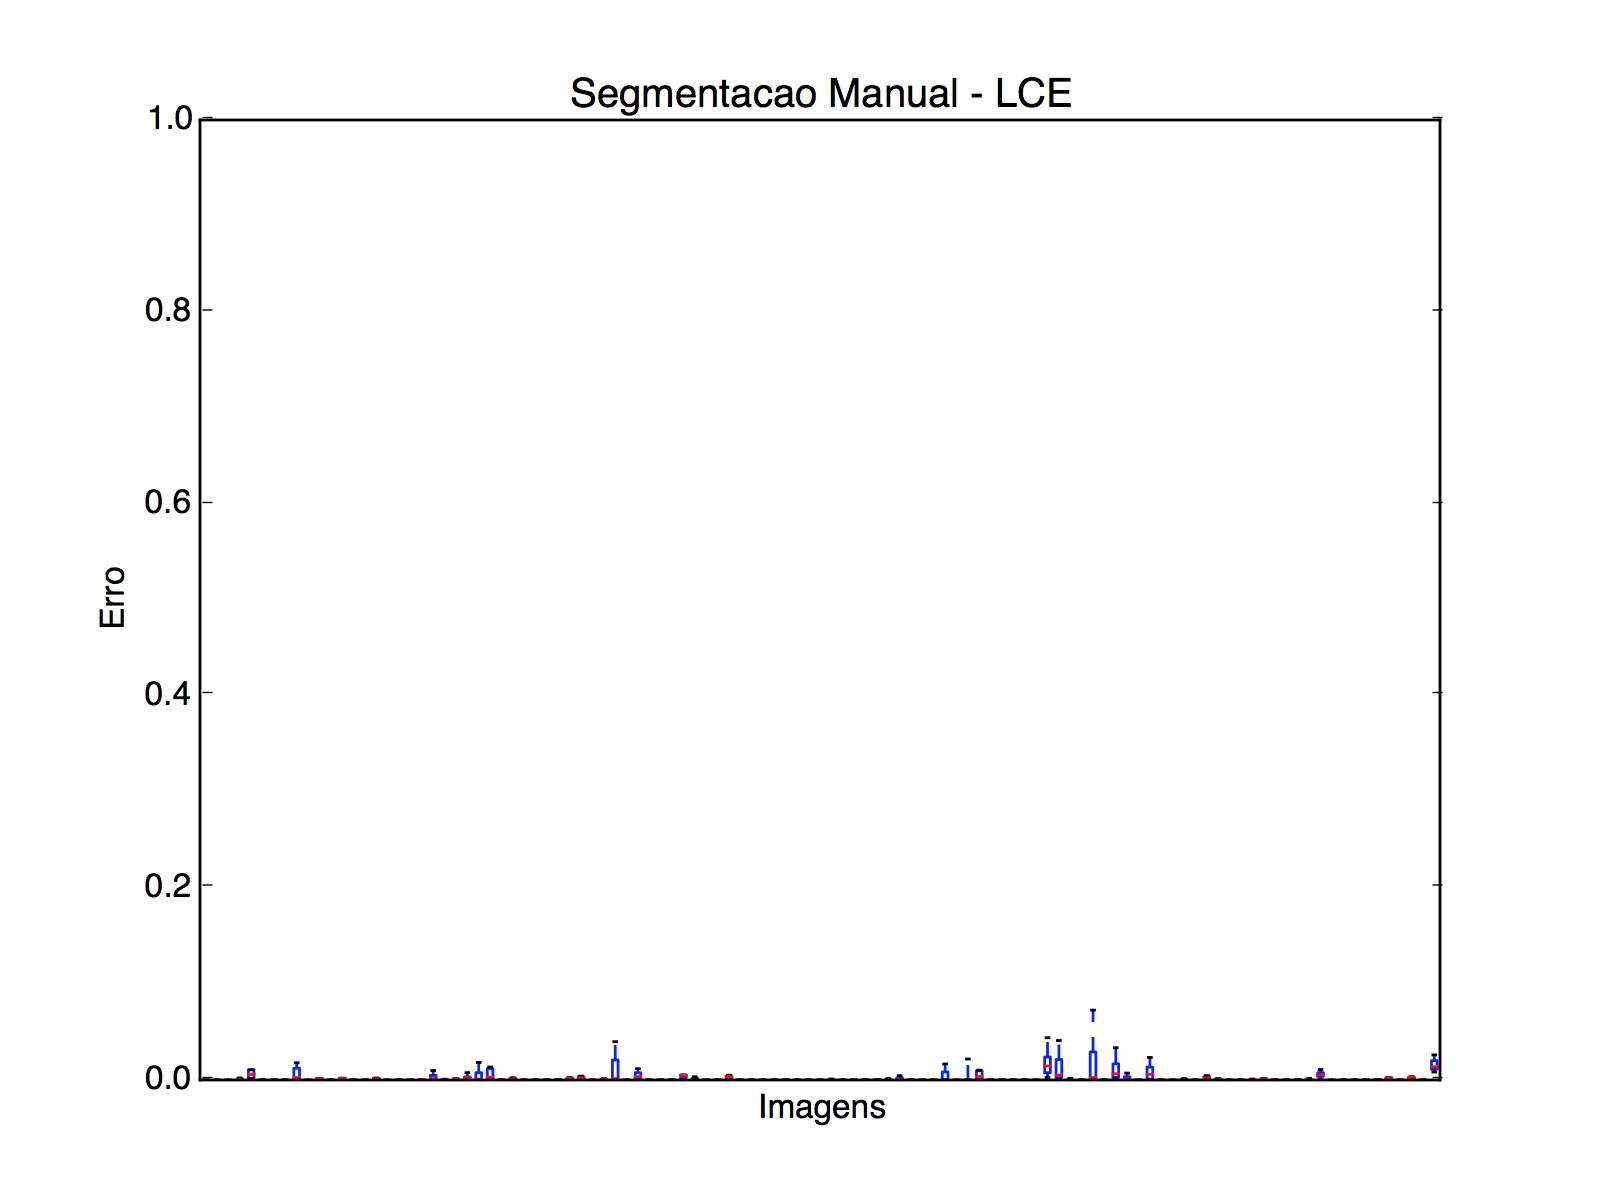
\includegraphics[width=\textwidth]{imgs/manual_dist_lce}
  \end{subfigure}%
  \caption{Coeficiente de erro local das diferentes segmentações de mesma imagem}
  \label{fig:manual_lce}
\end{figure}

Para determinar qual dos algoritmos de segmentação levantados na pesquisa bibliográfica teria melhor desempenho na base de dados utilizada neste trabalho, todos foram implementados ou adaptados. Os algoritmos foram testados em todas as imagens da base de dados do trabalho que possuíam segmentação manual por pelo menos 5 voluntários, um total de 203 imagens, utilizando as mesmas medidas de erro global (GCE) e erro local (LCE) apresentados no trabalho de \citeonline{martin:2001} e na validação da base de segmentação manual construída para este trabalho.

Os resultados do experimento são apresentados na tabela \ref{tab:experimentoSegmentacao}:

\begin{table}[h]
\ABNTEXfontereduzida
\centering
\begin{tabulary}{\linewidth}{|L|R|R|R|}
\hline
\textbf{Algoritmo} & \textbf{GCE médio} & \textbf{LCE médio} & \textbf{Tempo (s)} \\ \hline
Manual      & 0.01762          & 0.00525 & 6,39 \\ \hline
Mean-shift  & 0.02528          & 0.00278 & 6,39 \\ \hline
JSEG        & 0.03209          & 0.00532 & 14,82 \\ \hline
MSEG        & 0.00983          & \textbf{0.00070} & \textbf{0,33} \\ \hline
SRM         & \textbf{0.00792} & 0.00421 & 4,66 \\ \hline
gPb-owt-ucm & 0.00903 & 0.00397 & 237,32 \\ \hline
FSEG        & 0.03385 & 0.00278 & 13,91 \\ \hline
\end{tabulary}
\caption{Comparação de métodos de segmentação em parte da base de imagens deste trabalho, ordenados por acurácia}
\label{tab:experimentoSegmentacao}
\end{table}

Apesar de que o algoritmo MSEG tenha alcançado menor erro local (LCE) e tempo de execução uma ordem de magnitude mais rápido que os outros algoritmos, ficou aquém na média de erro global (GCE).

O método SRM conseguiu uma média de erro global pouco menor que o algoritmo MSEG e será considerado uma alternativa, embora o tempo de segmentação deste algoritmo seja consideravelmente maior. A imagem \ref{fig:comparacaoSegmentacao} mostra a saída de alguns dos métodos testados, para fins de comparação visual.

\begin{figure}[htb]
	\centering
	\begin{minipage}[l]{0.32\linewidth}
		\begin{subfigure}[b]{\linewidth}
			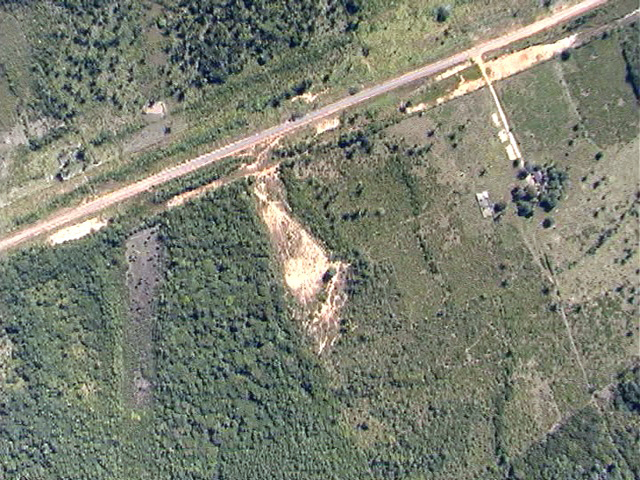
\includegraphics[width=\linewidth]{imgs/seg_original}
			\caption{Imagem original}
		\end{subfigure}%
	\end{minipage}
	\begin{minipage}[r]{\linewidth}
		\begin{subfigure}{.32\linewidth}
			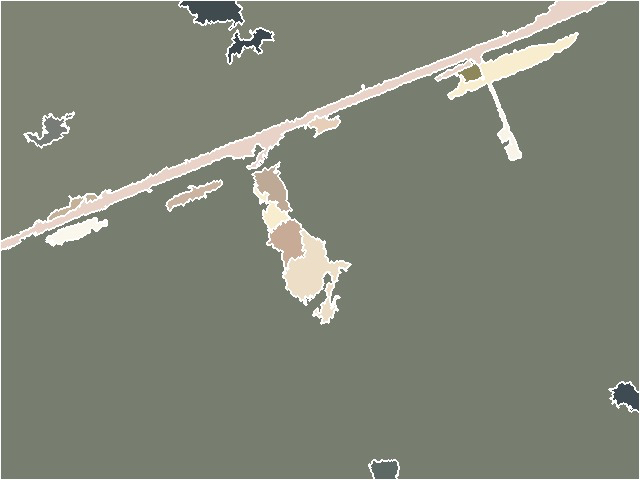
\includegraphics[width=\linewidth]{imgs/seg_meanshift}
			\caption{Mean-shift}
		\end{subfigure}
		\begin{subfigure}{.32\linewidth}
			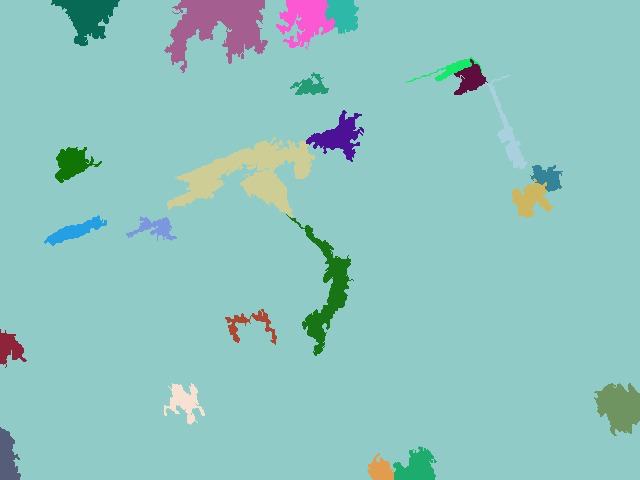
\includegraphics[width=\linewidth]{imgs/seg_mseg}
			\caption{MSEG}
		\end{subfigure}
		\begin{subfigure}{.32\linewidth}
			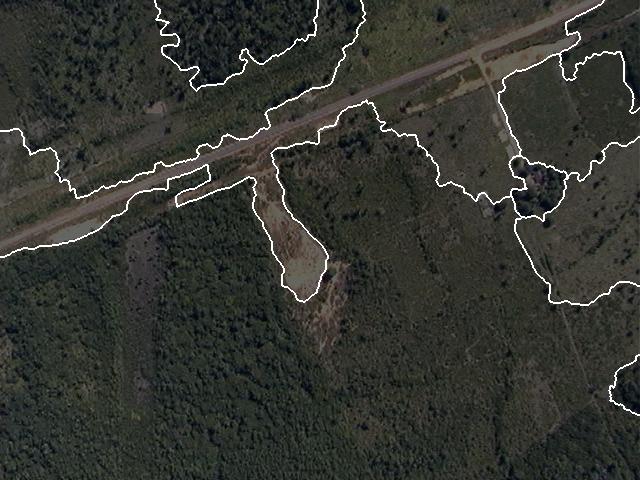
\includegraphics[width=\linewidth]{imgs/seg_jseg}
			\caption{JSEG}
		\end{subfigure}
	\end{minipage}
	\begin{minipage}[r]{\linewidth}
		\begin{subfigure}{.32\linewidth}
			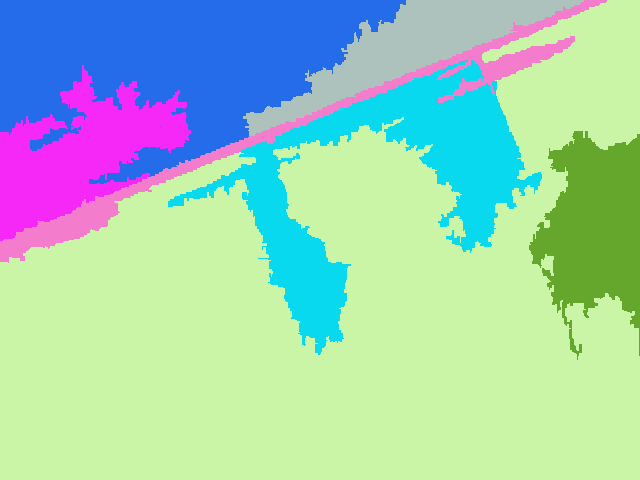
\includegraphics[width=\linewidth]{imgs/seg_srm}
			\caption{SRM}
		\end{subfigure}
		\begin{subfigure}{.32\linewidth}
			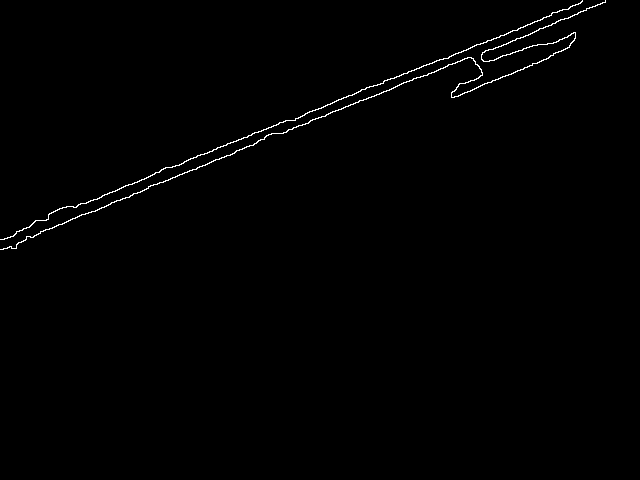
\includegraphics[width=\linewidth]{imgs/seg_gpb}
			\caption{gPb-owt-ucm}
		\end{subfigure}
		\begin{subfigure}{.32\linewidth}
			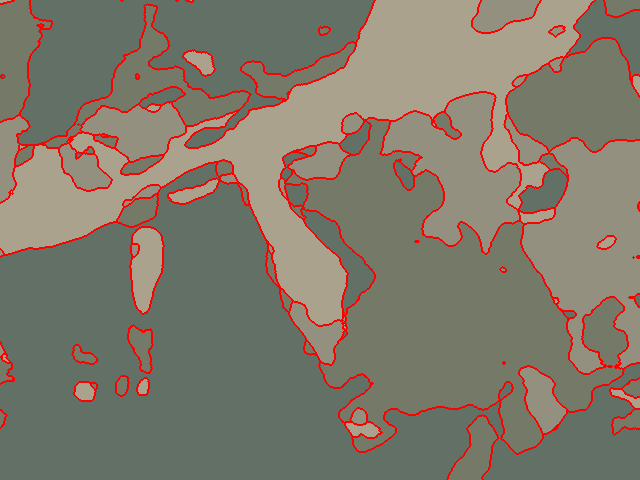
\includegraphics[width=\linewidth]{imgs/seg_fseg}
			\caption{FSEG}
		\end{subfigure}%
	\end{minipage}
	\caption{Comparação visual de métodos de segmentação}
	\label{fig:comparacaoSegmentacao}
\end{figure}


Adicionalmente, experimentos foram realizados com técnicas de classificação. O objetivo era saber se poderíamos utilizar apenas uma etapa para realizar segmentação e o primeiro nível de classificação. Os resultados foram abaixo do que se consegue na etapa de segmentação isolada. Os resultados foram publicados no \textit{$10^th$ International Conference on Computer Vision Theory and Applications} e o artigo \cite{cavalcanti:2015} completo pode ser visto no apêndice \ref{cap:visapp2015}.

Para fins de comparação, os resultados deste segundo experimento são apresentados na tabela \ref{tab:experimentoArtigo}. O tempo de execução da classificação para cada imagem no artigo publicado ignora o tempo de extração de características da imagem. Para uma comparação correta com os métodos de segmentação experimentados anteriormente, esse tempo gasto em extração de características foi acrescido na tabela desta seção.

\begin{table}[h]
\ABNTEXfontereduzida
\centering
\begin{tabulary}{\linewidth}{|L|R|R|}
\hline
\textbf{Algoritmo} & \textbf{Acurácia} & \textbf{Tempo/imagem} \\ \hline
Random forest  & 96,0\% & 12,72 s \\ \hline
KNN            & 92,6\% & 22,89 s \\ \hline
Naive Bayes    & 92,8\% & 8,36 s \\ \hline
Decision tree  & 82,2\% & 14,49 s \\ \hline
\end{tabulary}
\caption{Comparação de métodos de classificação para segmentação das imagens em uma única etapa, ordenados por acurácia}
\label{tab:experimentoArtigo}
\end{table}

Os segmentos encontrados pelo algoritmo escolhido nesta etapa serviu de entrada para a próxima etapa da solução, responsável pela classificações destes mesmos segmentos.

\section{Classificações de regiões}

Para o primeiro nível de classificação, que se resume a definir os tipos de terrenos das regiões encontradas na segmentação, um experimento com métodos bastante difundidos de aprendizagem de máquina foi realizado.

Utilizando as técnicas de K vizinhos mais próximos (KNN), máquinas de vetores de suporte (SVM) e árvores de decisão, um experimento foi conduzido em uma parte da base de dados. As mesmas 150 imagens do experimento de segmentação anteriormente apresentado foram utilizadas.

Primeiramente, todas as imagens foram segmentadas utilizando o método Mean-shift, por ter obtido o melhor desempenho no experimento de segmentação anterior. Cada região encontrada nesta segmentação foi devidamente classificada manualmente, e suas características foram extraídas. A partir desse ponto bases de dados de treinamento e validação supervisionadas foram criadas, onde cada região segmentada representava uma amostra de treinamento ou validação.

As características extraídas para cada região foram:
\begin{itemize}
	\item Cor média para os canais vermelho, verde e azul;
	\item Histograma dos canais vermelho, verde e azul;
	\item Tom de cinza médio;
	\item Histograma de tons de cinza.
\end{itemize}

Estas características foram escolhidas em primeira instância por serem de fácil extração, baixa dimensionalidade e simples depuração/verificação. Muitos dos trabalhos na literatura utilizam características de cor e histogramas em tons-de-cinza. Como um trabalho prospectivo, estas características foram consideradas bons pontos de partida.

O total de 7.111 amostras foram classificadas, onde 4.694 (66\%) foram utilizadas como amostras de treinamento e 2.417 (33\%) foram utilizadas como amostras de validação. O método SVM teve desempenho ligeiramente superior aos demais, como pode ser visto na tabela \ref{tab:experimentoClassificacao1}, que apresenta os resultados de acurácia, precisão, e revocação para os métodos analisados.

\begin{table}[h]
\ABNTEXfontereduzida
\centering
\begin{tabulary}{\linewidth}{|L|R|R|R|}
\hline
\textbf{Método} & \textbf{Acurácia} & \textbf{Precisão} & \textbf{Revocação} \\ \hline
SVM               & 89,19\% & 0,927 & 0,864 \\ \hline
KNN               & 88,51\% & 0,912 & 0,863 \\ \hline
Árvore de decisão & 87,09\% & 0,842 & 0,859 \\ \hline
\end{tabulary}
\caption{Comparação de métodos de classificação para regiões segmentadas das imagens, ordenados por acurácia}
\label{tab:experimentoClassificacao1}
\end{table}

Embora os resultados tenham sido promissores, ainda há bastante espaço para melhoria. Apenas características de cor e luminância foram exploradas, portanto, características de textura, morfologia e borda ainda precisam ser avaliadas.


\section{Próximos passos}

Para os próximos meses de pesquisa, diversas características serão extraídas e avaliadas para o primeiro nível de classificação:

\begin{itemize}
	\item Bordas;
	\item Textura;
	\item Morfologia;
	\item Bag of visual words
	\item Vizinhança de regiões.
\end{itemize}

Além disso, técnicas ensembles de classificadores também serão avaliados e comparados com os resultados atuais.

Para a fase final de classificação, será feito um levantamento de características e algoritmos de classificação para a detecção de elementos anômalos dentro das regiões segmentadas. Nesta fase serão explorados classificadores unitários (\textit{one-class classifiers}), visto que a literatura relata bons resultados com este tipo de classificador para detecção de anomalias e \textit{outliers}. Após estes experimentos, todo o fluxo de classificação será reavaliado, a fim de otimizar a taxa de aprendizado e generalização dos classificadores.

Por fim, o volume final da dissertação de mestrado será composto, levando em consideração os melhores resultados dos experimentos. Artigos também serão feitos e submetidos, refletindo partes relevantes da pesquisa e seus resultados.
